\chapter{Experiments}\label{ch:experiments}
This chapter covers the most important experiments that we have conducted. Along with that, we provide details on how we proceeded and also some thought processes that influenced our decisions. At the end of this chapter, we present a summary of our results.

\section{Benchmark setup}
The goal of this thesis is to benchmark the performance of multiple ansatzes and optimizers. Potentially, find some intriguing relationships from data created from many VQE runs. \todo{this is at odds with the thesis assignment}. The first thing that came to our mind was to take a few optimizers and ansatzes and so we can see how they perform. We did that by plotting an energy convergence graph. We discovered that the performance of VQE highly depends on chosen optimizers. 

\begin{figure}[H]
    \centering
    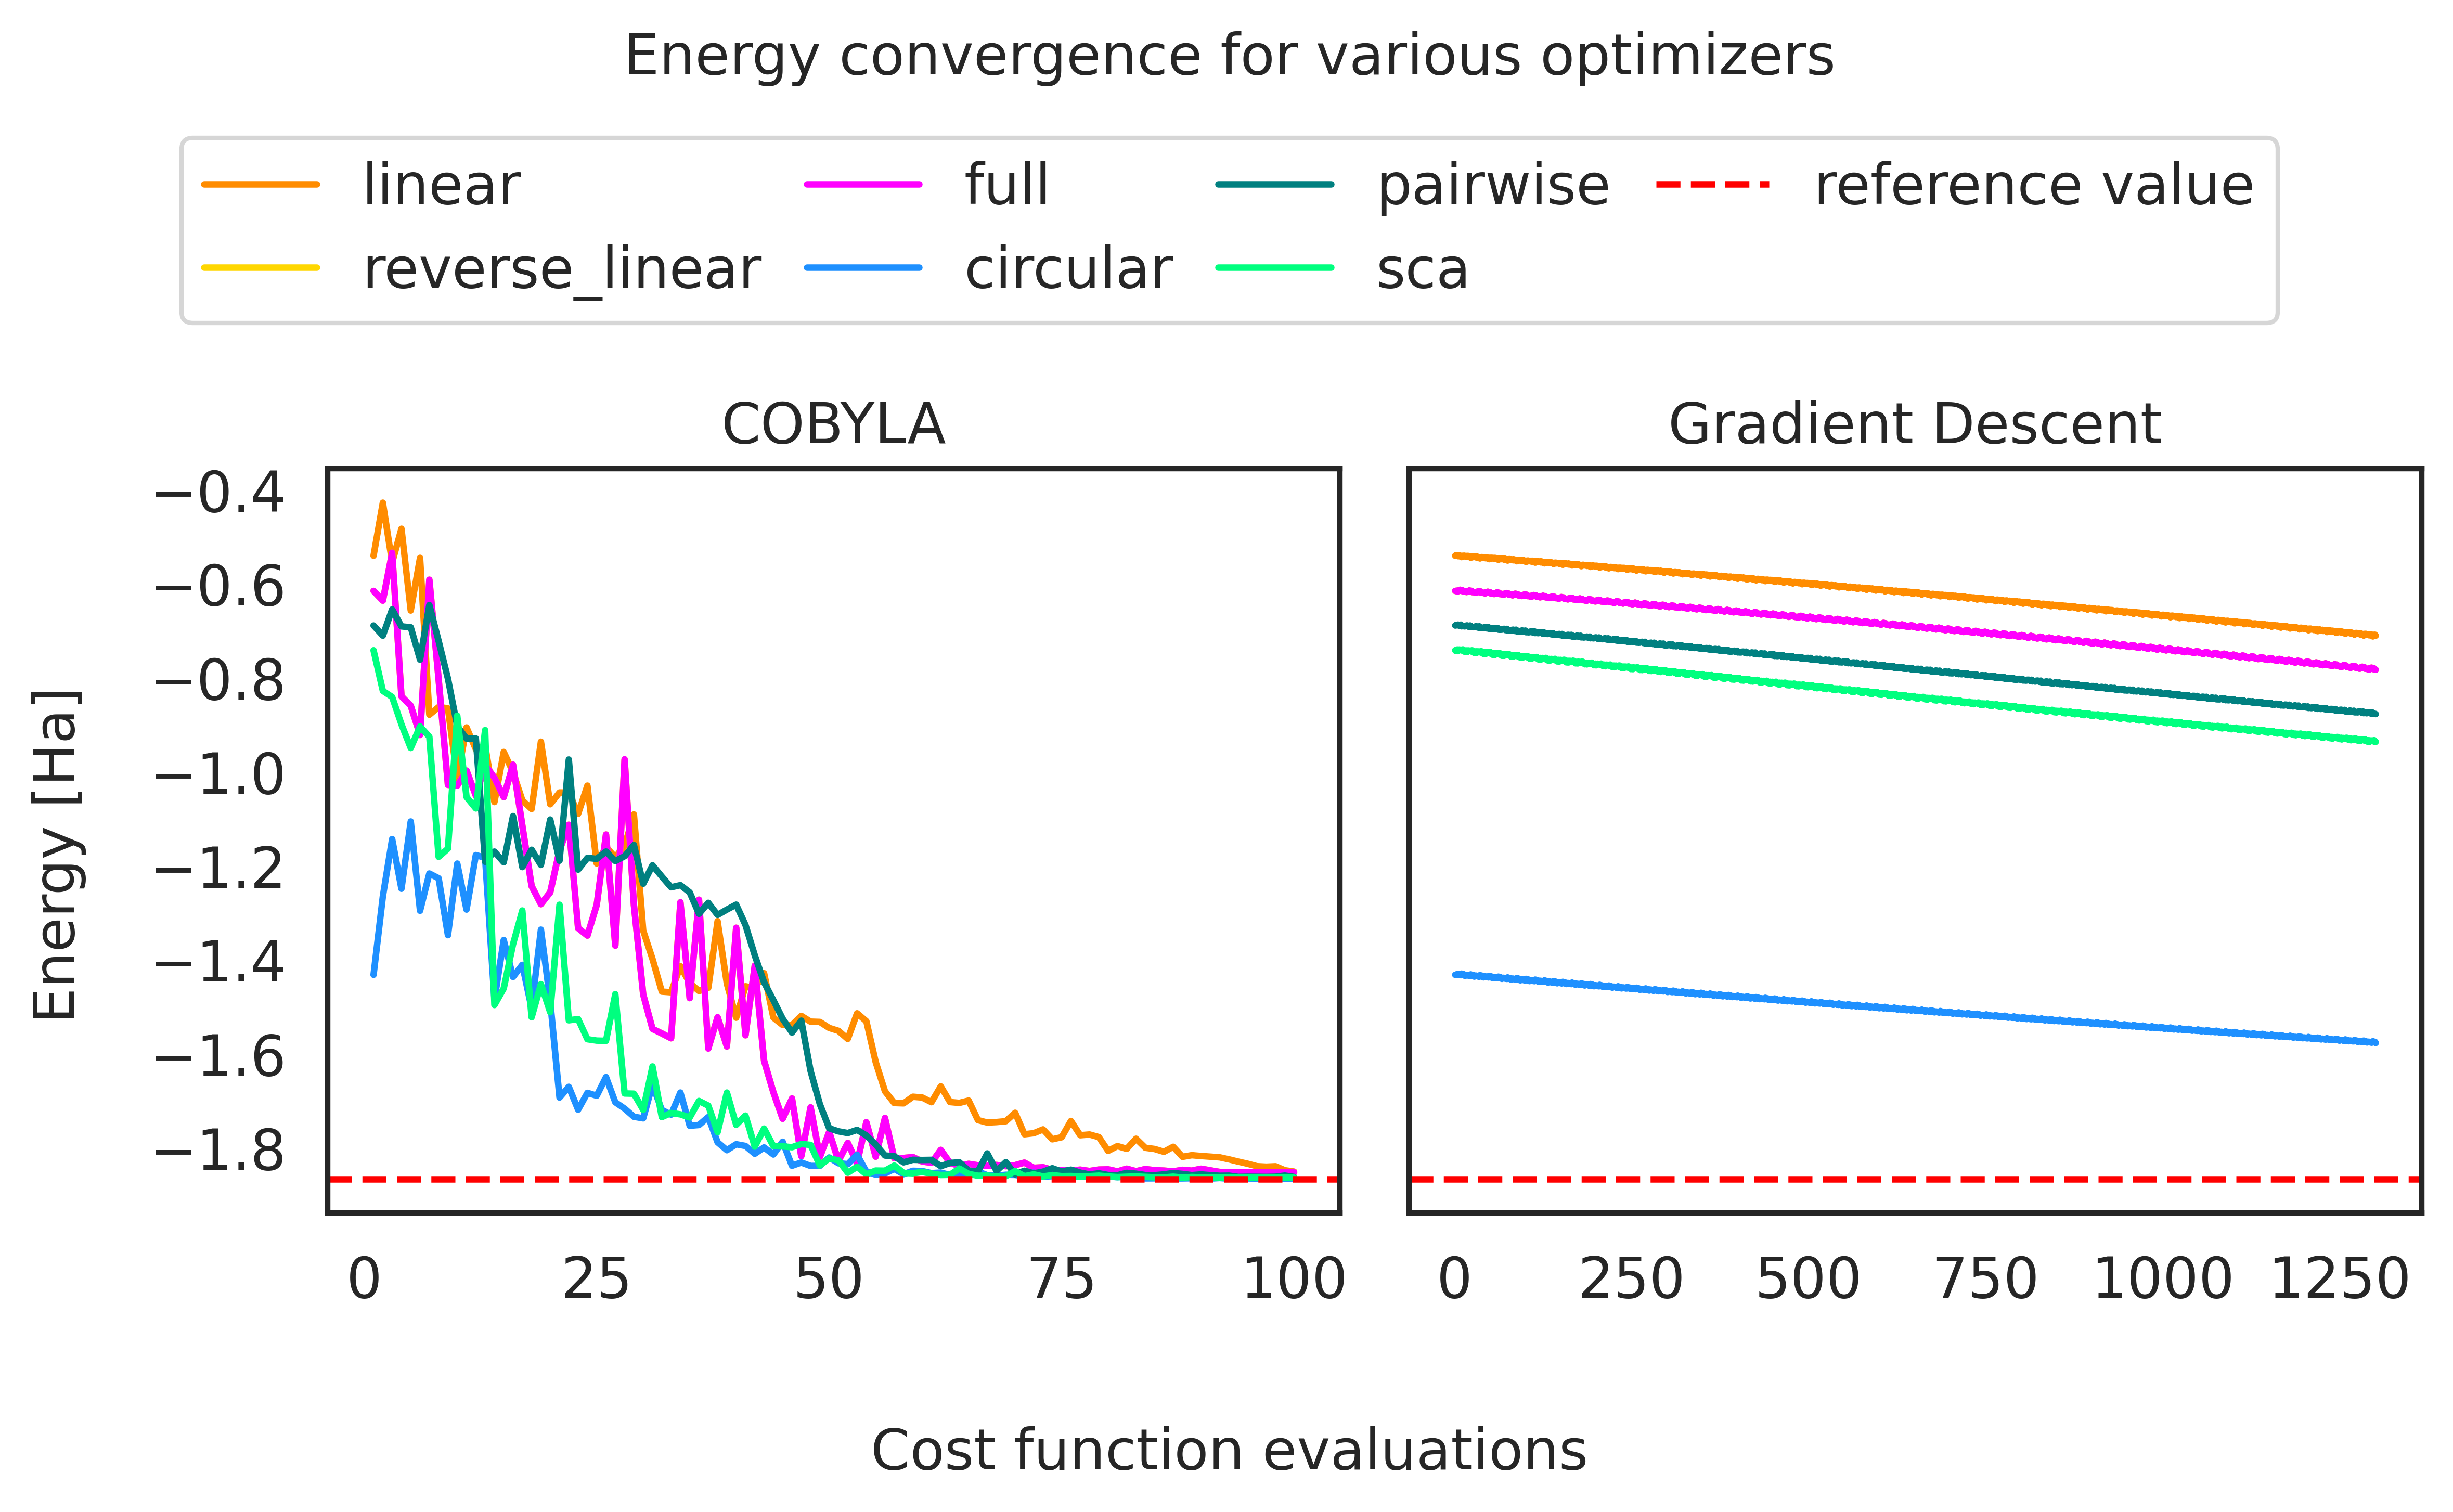
\includegraphics[width=\textwidth]{convergence_example.png}
    \caption{Exmaples of energy convergence for various optimizers}
    \label{fig:energy-convergence}
\end{figure}

In figure \ref{fig:energy-convergence} we can observe that not only energy convergence but also cost function evaluations differ a lot. Some optimizers have a fixed number of cost function evaluations for each iteration, and some of them can use an arbitrary number of cost function evaluations. \todo{verify whether it is really arbitrary} Another thing worth pointing out is that we benchmarked six ansatzes, however, we can see only five of them. The reverse linear ansatz is overlapped by the full ansatz since a matrix representation of the reverse linear ansatz is the same as the full ansatz. All the disparities led us to create a more complex benchmark that includes multiple ansatzes and optimizers.

\subsubsection{Ansatzes}
In our benchmark, we categorized ansatzes based on entanglement. We decided to go with 6 ansatzes, namely linear, reverse linear, full, circular, pairwise, and SCA. From each ansatz, we have created 3 variations, 1 layer, 2 layers, and 3 layers ansatzes. In total, we have 18 parametrized quantum circuits that we tried to run a VQE algorithm on.

\subsubsection{Optimizers}
After browsing some scientific articles we have not found any definite answer to which optimizers work the best. For that reason, we decided to test almost all optimizers that Qiskit offers. \todo{maye mention why I excluded P\_BFGS\_B and GSLS algorithms} Also, the optimizers offer a plethora of hyperparameters (parameters used to configure the optimizers themselves) and configuring them would be a nightmare so we went with the default ones, except for the number of iterations. We set the number of iterations to 100 for each optimizer. In the table~\ref{tab:optimizers} below we can see all the optimizers that we tested.

\begin{table}[H]
    \centering
    \begin{tabular}{|l|c|c|} 
        \hline
        \multicolumn{1}{|c|}{\textbf{Optimizer}} & \textbf{Type}\\
        \hline
        AQGD (Analytical Quantum Gradient Descent) & gradient-free \\ 
        \hline
        NFT (Nakanishi-Fujii-Todo) & gradient-free \\ 
        \hline
        QNSPSA (Quantum Natural SPSA) & gradient-free \\ 
        \hline
        SPSA (Simultaneous Perturbation Stochastic Approximation) & gradient-free \\ 
        \hline
        COBYLA (Constrained Optimization By Linear Approximation) & gradient-free \\ 
        \hline
        Nelder Mead & gradient-free \\ 
        \hline
        Powell & gradient-free \\ 
        \hline
        UMDA (Continuous Univariate Marginal Distribution Algorithm) & gradient-free \\ 
        \hline
        Gradient Descent & gradient-based \\ 
        \hline
        CG (Conjugate Gradient) & gradient-based \\ 
        \hline
        ADAM (Adaptive Moment Estimation) & gradient-based \\ 
        \hline
        AMSGRAD (a variant of ADAM with memory) & gradient-based \\ 
        \hline
        L\_BFGS\_B (Limited-memory BFGS Bound)  & gradient-based \\ 
        \hline
        SLSQP (Sequential Least SQuares Programming)  & gradient-based \\ 
        \hline
        TNC (Truncated Newton)  & gradient-based \\ 
        \hline
    \end{tabular}
    \caption{Tested optimizers}
    \label{tab:optimizers}
\end{table}

\subsubsection{Hamiltonian}
For all the experiments we used a 4-qubit Hamiltonian of a hydrogen molecule. We took it from a paper produced by Miháliková et al.~\cite{mihalikova} and it is defined as follows:

\begin{align*}H_{H_2}^{4-qubit} &= c_{0}1 + c_{1}Z_{0} + c_{2}Z_{1}Z_{0} + c_{1}Z_{2} + c_{2}Z_{3}Z_{2}Z_{1} + c_{3}Z_{1} + c_{4}Z_{2}Z_{0}\\
                                &+ c_{5}X_{2}Z_{1}X_{0} + c_{6}Z_{3}X_{2}X_{0} + c_{6}X_{2}X_{0} + c_{5}Z_{3}X_{2}Z_{1}X_{0}\\
                                &+c_{7}Z_{3}Z_{2}Z_{1}Z_{0} + c_{7}Z_{2}Z_{1}Z_{0} + c_{8}Z_{3}Z_{2}Z_{0} + c_{3}Z_{3}Z_{1},
\end{align*}
where coefficients are as follows:
\begin{alignat*}{3}
    &c_0 = -0.80718,\qquad &c_1 = 0.17374,\qquad &c_2 =-0.23047, \\
    &c_3 = 0.12149,\qquad  &c_4 = 0.16940,\qquad &c_5 = -0.04509, \\
    &c_6 = 0.04509,\qquad  &c_7 = 0.16658,\qquad &c_8 = 0.17511.
\end{alignat*}

This Hamiltonian can be further simplified to 2 qubits, however, we have retained this form to make the problem a little bit more complex. The ground state of this Hamiltonian is $-1.8671050114542505$, we calculated that using a \textit{NumPyMinimumEigensolver} algorithm provided by Qiskit and we will use this value as a reference value for our experiments.

\subsubsection{Implementation and data exploration}
For all the experiments we used the Qiskit library, therefore all our code was written in Python programming language. Due to Python's global interpreter lock (GIL) that allows the execution of only a single thread at a time, we were forced to use Python's multiprocessing module. To speed up our computations we created multiple processes, each process was responsible for a single optimizer and these processes are automatically distributed to available CPU cores.

All the data that we collected from VQE runs we saved into a CSV file. This allowed us to later load the data into a Pandas data frame and perform some data exploration. For data exploration, we primarily leveraged the Plotly library which has an easy to use API and creates nice interactive visualizations with few lines of code. However, all the visualizations included in this thesis were created using Seaborn library, which is built on top of Matplotlib. All the code that we created for this thesis is available on GitHub. \todo{check whether it needs to be in appendix}

It is important to mention that all computations we are considering here are ideal, meaning that we are not taking into account any noise. Together we have 15 optimizers and 18 ansatz, which means we have 270 combinations total on how we can run VQE. We ran each combination 50 times and each time with different initial points provided to ansatz. 

\section{Results} 
Initially, after we had run all the experiments, we were interested again in energy convergence, so we plotted an extensive graph that shows how the energy convergence for each optimizer and ansatz. After exploring all graphs, it seemed that gradient-free optimizers are doing better and they can converge faster. However, such an amount of data is difficult to read and infer some conclusions from it. Therefore, we decided to introduce a new figure of merit. We consider the probability of reaching a chemical accuracy. Chemical accuracy refers to how closely individual measurements agree with the correct, or ''true'', value~\cite{chemistry}. A chemical accuracy for a hydrogen molecule is $0.0016Ha$ \todo{cite this fact}. \ques{should it be accuracy or precision? I cited that from a chemistry book and to me it seems that accuracy is the right term but I may be mistaken}


The first important thing that we have discovered is that it is impossible to reach a chemical precision with a 1-layer ansatz for any optimizer.
\begin{figure}[H]
    \centering
    \includegraphics[width=\textwidth]{layers.png}
    \caption{Impact of ansatz layers}
    \label{fig:ansatz-layers}
\end{figure}

In Figure \ref{fig:ansatz-layers}, we can see that no matter the optimizer, the probability of reaching a chemical precision is always zero for a 1-layer ansatz. Another very interesting thing is that gradient-based optimizers perform better with 3-layer ansatzes and gradient-free optimizers perform better with 2-layer ansatzes. We believe that this could be due to the number of parameters that need to be optimized. For all the subsequent visualizations, we ditched the 1-layer ansatzes and focused only on 2 and 3-layer ansatzes.

\begin{figure}[H]
    \centering
    \includegraphics[width=\textwidth]{chemical.png}
    \caption{Probability of reaching chemical precision for various optimizers, ansatzes, and number of layers}
    \label{fig:chemical}
\end{figure}
\todo{fix title, it is too long and it does not fit here, crop the top and bottom whitespace}

The figure above can seem a bit unclear due to the amount of overlapping data points. However, we can observe that the best results were achieved by some of the gradient-based optimizers, namely \textit{Conjugate Gradient}, \textit{L\_BFGS\_B} and \textit{SLSQP}. Gradient-free optimizers perform worse and they are more dependent on chosen ansatz whereas gradient-based optimizers tend to reach a very good probability no matter the ansatz, or they do not work at all. 

\begin{figure}[H]
    \centering
    \includegraphics[width=\textwidth]{evaluations.png}
    \caption{Cost function evaluations along with the probability of reaching chemical perecision}
    \label{fig:evaluations}
\end{figure}

If we look at the number of cost function evaluations, we can deduce some guesses why some of the algorithms do not perform well. The straight lines that we can see on \textit{NFT}, \textit{QNSPSA}, \textit{SPSA}, \textit{COBYLA}, \textit{ADAM}, and \textit{AMSGRAD} mean that these optimizers have a fixed number of cost function evaluations. It seems that a fixed number of cost function evaluations can have a limiting impact on the optimizers. Multiple optimizers that have a smaller number of cost function evaluations are not very likely to reach a chemical precision.

However, we can not generalize that, \textit{L\_BFGS\_B} and \textit{SLSQP} reached very good results despite the lower number of cost function evaluations. On the other hand, \textit{Gradient Descent} and \textit{TNC} algorithms do not work at all even though the number of cost function evaluations is not so small. The \textit{Conjugate Gradient} has the best probability overall but it costs us a lot of cost function evaluations. Strikingly, this algorithm uses the same principle as an ordinary \textit{Gradient Descent} but to make a decision it uses past decisions.

As clear winners seem \textit{L\_BFGS\_B} and \textit{SLSQP}, both of them are quasi-Newton. They have a very high probability of reaching a chemical precision, a smaller number of cost function evaluations and they were able to reach a chemical precision with all tested ansatzes without any significant difference in results. Nevertheless, the best optimizer can vary from the situation, sometimes we can strive to minimize the number of cost function evaluations since at the end of the day it is what we pay for. We believe that many of the optimizers could perform better if we tuned their hyperparameters. Especially for the optimizers with a fixed number of cost function evaluations, increasing the number of iterations could help.


\todo{v tejto casti je to mozno take pribehovejsie a je tam akasi casova os, mato byt tak alebo mam radsej len povedat, ze toto su vysledky ale ten nas myslienkovy proces ako sme sa k nim dostali je zbytocny?}